\documentclass{prepareprotokol} %všechny balíčky pro protokol + titulní strana
\usepackage{amsmath}

%\usepackage[cp1252,<other encodings>]{inputenc}
\makeatletter
\def\fnum@figure{Graf \thefigure}
\makeatother
\usepackage[version=4]{mhchem}
\usepackage{adjustbox}
\usepackage{booktabs}
\usepackage{hyperref}
\usepackage{makecell}  % Na zvýšenie riadkov
\usepackage{array}     % Na tabuľky s vlastnými stĺpcami
\usepackage{epsfig}				% Obrázky ve vektorovém formátu EPS
\usepackage{indentfirst}		% České odsazení prvního odstavce 
\usepackage{boldline}
\usepackage{graphicx}
\usepackage{mhchem}
\usepackage{color}
\usepackage{caption}
\usepackage{subcaption}
\usepackage{amsmath}
\usepackage{amssymb}
\usepackage{float}
\praktikum{I} %číslo praktika (I, II nebo III)
\autor{Lukáš Jarábek} %jméno autora
\datum{1.\,4.\,2025} %datum měření
\cislo{VI} %číslo úlohy
\nazev{Štúdium reologického chovania látok  

DU Práca s Počítačmi} %název úlohy

\begin{document}
	\maketitle
	\let\oldref\ref
	\renewcommand{\ref}[1]{(\oldref{#1})}
	\newcommand{\Nm}{$\mbox{N}\cdot\mbox{m}^{-2}$}
	\newcommand{\ms}{$\mbox{m}\cdot\mbox{s}^{-2}$}
	\newcommand{\kgm}{$\mbox{kg}\cdot\mbox{m}^{-3}$}
	
	
\section*{Pracovná úloha}
\begin{enumerate}
\item Pre newtonovskú kvapalinu (glycerín) študujte ustálený systém pri meraní rotačným viskozimetrom - zmerajte časovú závislosť viskozity pre rôzne rýchlosti deformácie.
\item Odhadnite chybu merania viskozity pre rôzne rýchlosti deformácie (na základe úlohy 1).
\item Zmerajte tokovú krivku pre glycerín pre niekoľko teplôt.
\item Zmerajte teplotnú závislosť viskozity glycerínu v obore teplôt od 10 °C do 40 °C. Určite aktivačnú energiu.
\item V manuálnom režime určite rozsah použiteľnej rýchlosti deformácie pre škrob (pri pokojovej teplote).
\item Zmerajte tokovú krivku pre nenewtonskú kvapalinu (škrob alebo tekuté mydlo) pri konštantnej teplote.
\item Pyknometrickou metódou určite hustotu glycerínu a stanovte podiel vody v glyceríne.
\end{enumerate}
	
\section*{Teória}
        
Chovanie viskóznej tekutiny popisujeme rovnicou toku, ktorá je podľa \cite{Študijný text}

\begin{equation}
		\tau = f(\dot{\gamma}),
		\label{eq:RovnicaToku}
\end{equation} 

kde $\tau$ je šmykové napätie a $f(\dot{\gamma})$ je funkčná závislosť rýchlosti šmykovej deformácie.\\

Pokiaľ je táto funkčná závislosť lineárna a je popísaná rovnicou

\begin{equation}
		\tau = \eta\dot{\gamma},
		\label{eq:Newtonovska}
\end{equation} 

tak tekutinu nazývame newtonovskou. 
$\eta$ v tejto rovnici reprezentuje dynamickú viskozitu tekutiny.\\

Nenewtonovské tekutiny sú také tekutiny, pre ktoré lineárna závislosť vo vzorci \ref{eq:Newtonovska} neplatí. 
Dokážeme teda rozpoznať nenewtonovskú tekutinu vtedy, ak systematická odchýlka viskozity počítanej podľa vzťahu \ref{eq:Newtonovska} bude prevyšovať chybu prístroja.\\

Dynamická viskozita popisuje prenos hybnosti medzi dvoma susednými vrstvami tekutiny realizovaný pomocou molekúl. 
Preto viskozita je závislá od teploty a túto závislosť vieme podľa \cite{Študijný text} popísať ako

\begin{equation}
		  \eta = C\mathrm{exp}(\frac{\varepsilon_a}{kT}),
		\label{eq:TeplotnaZavislost}
\end{equation} 

kde $T$ popisuje termodynamickú teplotu, $\varepsilon_a$ aktivačnú energiu, $k$ Boltzmannovu konštantu a $C$ je konštanta.\\

Na meranie reologického správania látok používame rotačný viskozimeter. 
Takýto typ viskozimetra meria odpor, ktorý kladie tekutina rotujúcemu telesu, ktoré je ponorené do tejto tekutiny. 
Toková krivka zodpovedá závislosti šmykového napätia od rýchlosti šmykovej deformácie.\\


Počas merania skúmame glycerín, ktorý má sumárny vzorec $\mathrm{C}_3\mathrm{H}_8\mathrm{O}_3$. Glycerín má $3~\mathrm{OH}$ skupiny, ktoré budú tvoriť vodíkové mosty, ktoré budú spôsobovať vysokú viskozitu. 
To si vieme predstaviť tak, že keďže glycerín obsahuje vodíkové mosty, tak zvýši počet interakcii medzi molekulami, ktoré budú spomaľovať makroskopický tok tejto kvapaliny, čo sa prejaví na vyššej viskozite. 
Avšak pri zvyšovaní teploty sa tieto väzby budú roztrhávať, keďže ide o slabé väzby, kvôli čomu sa bude znižovať viskozita. \\

Takisto meriame škrob, ktorý je nenewtonovská látka.
Podľa \cite{Skrob} viskozita škrobu klesá pri vyšších rýchlostiach šmykovej deformácie. 
Podľa \cite{Hysteréza} pri škrobe sa prejavuje hysteréza systému, čo je vlastnosť systému, pri ktorom sa mení stav systému, vzhľadom na jeho históriu zmien stavov systému.\\

Je ale dôležité si uvedomiť, že glycerín je hygroskopická tekutina, čo znamená že absorbuje vodu z okolia, čiže zlúčenina takmer isto nebude čistý glycerín. 
Jeho koncentráciu preto môžeme zistiť pomocou hustoty zlúčeniny glycerínu pri pokojovej teplote, ktorú zmeriame pomocou pyknometrickej metódy. 
Počas tejto metódy najprv zmeriame pomocou digitálnych váh hmotnosť pyknometru aj s uzáverom, ktorú značíme $m_1$, potom doplna nalejeme referenčnú tekutinu s hustotou $\rho_1$ do pyknometra a zmeriame jej hmotnosť aj s pyknometrom značenú ako $m_2$.
Nakoniec vylejeme vodu, osušíme pyknometer a nalejeme doplna glycerín a zmeriame jeho hmotnosť aj s pyknometrom a túto hmotnosť budeme značiť $m_3$. 
Ako referenčnú tekutinu volíme destilovanú vodu.
Hustotu glycerínu $\rho_2$ pri pokojovej teplote potom vypočítame ako 

\begin{equation}
		  \rho_2 = \frac{m_3-m_1}{m_2-m_1}\rho_1.
		\label{eq:Pyknometer}
\end{equation} 



\section*{Postup merania a použité prístroje}
        
 Na začiatku sme zapli rotačný viskozimeter \textbf{HAAKE Viscotester iQ (Thermo scientific)}, pomocou ktorého sme študovali reologické správanie tekutín. 
 Tento prístroj bol napojený na program \textbf{HAAKE RheoWin Job Manager}, ktorý nám spracovával údaje z rotačného viskozimetra. 
 Tento rotačný viskozimeter nám zároveň ukázal pokojovú teplotu. 
 Z dokumentácie sme našli jeho neistotu určenia teploty ako $\pm~0,1~^\circ \mathrm{C}$. \\

Pri meraní sme používali dva súosé valce, ktoré sme neskôr umiestnili do rotačného viskozimetra, kde vnútorný valec rotoval v kvapaline, ktorá bola umiestnená vo vonkajšom valci. 
Vonkajší valec bol typu CC25 a vnútorný valec CCB25.
Pred meraním sme už mali nakalibrovaný rotačný viskozimeter. \\

Potom sme pomocou injekčnej striekačky naliali do vonkajšieho valca $17~\mathrm{ml}$ glycerínu. 
Neistotu určenia objemu injekčnou striekačkou určíme ako polovicu najmenšieho dielika, čo je $\pm~ 0,5~\mathrm{ml}$.\\

Následne sme tento glycerín vložili do rotačného viskozimetra, potom vnútorný valec, a uzavreli sme tento rotačný viskozimeter. 
Následne sme nastavili parametre merania, pričom sme nastavili, aby nám program \textbf{HAAKE RheoWin Job Manager} vyhodnotil skokový graf závislosti dynamickej viskozity a šmykového napätia od času pri teplote, ktorú sme nastavili na $20~^\circ \mathrm{C}$. 
Počas priebehu tohoto merania sme menili rýchlosť šmykovej deformácie. 
Z tohoto grafu sme určili chybu merania dynamickej viskozity ako najväčšiu amplitúdu výkyvov pri tej rýchlosti šmykovej deformácie, kde tie výkyvy prevyšovali výkyvy u ostatných rýchlostiach.\\

Potom sme urobili merania, kde sme nastavili teploty na $20~^\circ \mathrm{C}$ a $30~^\circ \mathrm{C}$, pričom sme nechali parametre v programe rovnaké, až na to, že sme nastavili, aby nám program vyhodnotil tokovú krivku glycerínu ako závislosť šmykového napätia a dynamickej viskozity od rýchlosti šmykovej deformácie. 
Takisto sme nastavili, aby graf bol na  logaritmickej škále, pretože pri lineárnej by hodnoty boli neprehľadné. 
Logaritmickú škálu odteraz budeme nazývať log--log škála.\\

Potom sme následne nastavili, aby nám program vyhodnotil závislosť dynamickej viskozity od teploty. 
Z tohoto grafu sme následne určili aktivačnú energiu. \\

Potom sme rozobrali valce z rotačného viskozimetra, dôkladne ich prečistili a naliali do nich pomocou injekčnej striekačky $17~\mathrm{ml}$ škrobu. 
Potom sme rovnakým spôsobom škrob vložili do rotačného viskozimetra a pri pokojovej teplote zmerali tokovú krivku škrobu. 
Tento graf bude tiež v log--log škále.\\

Takisto sme zmerali časovú závislosť dynamickej viskozity a šmykového napätia škrobu pre rôzne rýchlosti šmykovej deformácie a z tejto závislosti sme určili rozsah použiteľnej rýchlosti šmykovej deformácie.\\

Nakoniec sme pyknometrickou metódou určili pomocou digitálnych váh hustotu glycerínu, z čoho sme pomocou tabuliek zistili koncentráciu vody v glyceríne.
Neistota určenia hmotnosti pomocou digitálnych váh je $\pm~0,001~\mathrm{g}$.



\newpage
\section*{Výsledky merania}
\subsection*{Meranie tokových kriviek pre glycerín}

Pokojovú teplotu sme namerali ako $24,3(1)~^\circ \mathrm{C}$.
Vzhľadom na povahu merania sú ostatné počiatočné podmienky nevýznamné a iba minimálne ovplyvnia naše meranie a preto ich vplyv na experiment budeme uvažovať ako zanedbateľný.

Napriek tomu, že meranie objemu pomocou injekčnej striekačky nesie zo sebou neistotu určenia objemu, budeme považovať tento objem za presný, pretože sme po naliatí vložili do valca odmerku, ktorá mala zistiť, či bolo do valca naliate presné množstvo tekutiny pomocou toho, že sa iba špička tejto odmerky namočila do tekutiny.

Následne sme nastavili teplotu vzorky na $20~^\circ \mathrm{C}$ a pomocou programu \textbf{HAAKE RheoWin Job Manager} sme urobili skokový graf závislosti dynamickej viskozity a šmykového napätia od času. Z dokumentácie prístroja sme zistili, že neistota určenia teploty vo vnútri rotačného viskozimetra je $\pm~ 0,01~^\circ \mathrm{C}$, čo je zanedbateľná neistota voči ostatným neistotám, čiže ju naďalej v meraní nebudeme uvažovať. 
Táto závislosť je obsiahnutá v grafe \ref{fig:sub1}, ktorý sme urobili pomocou programu \textbf{Origin}. Pomocou tohoto programu sme urobili aj všetky ostatné grafy.

\begin{figure}[H]
    \centering
    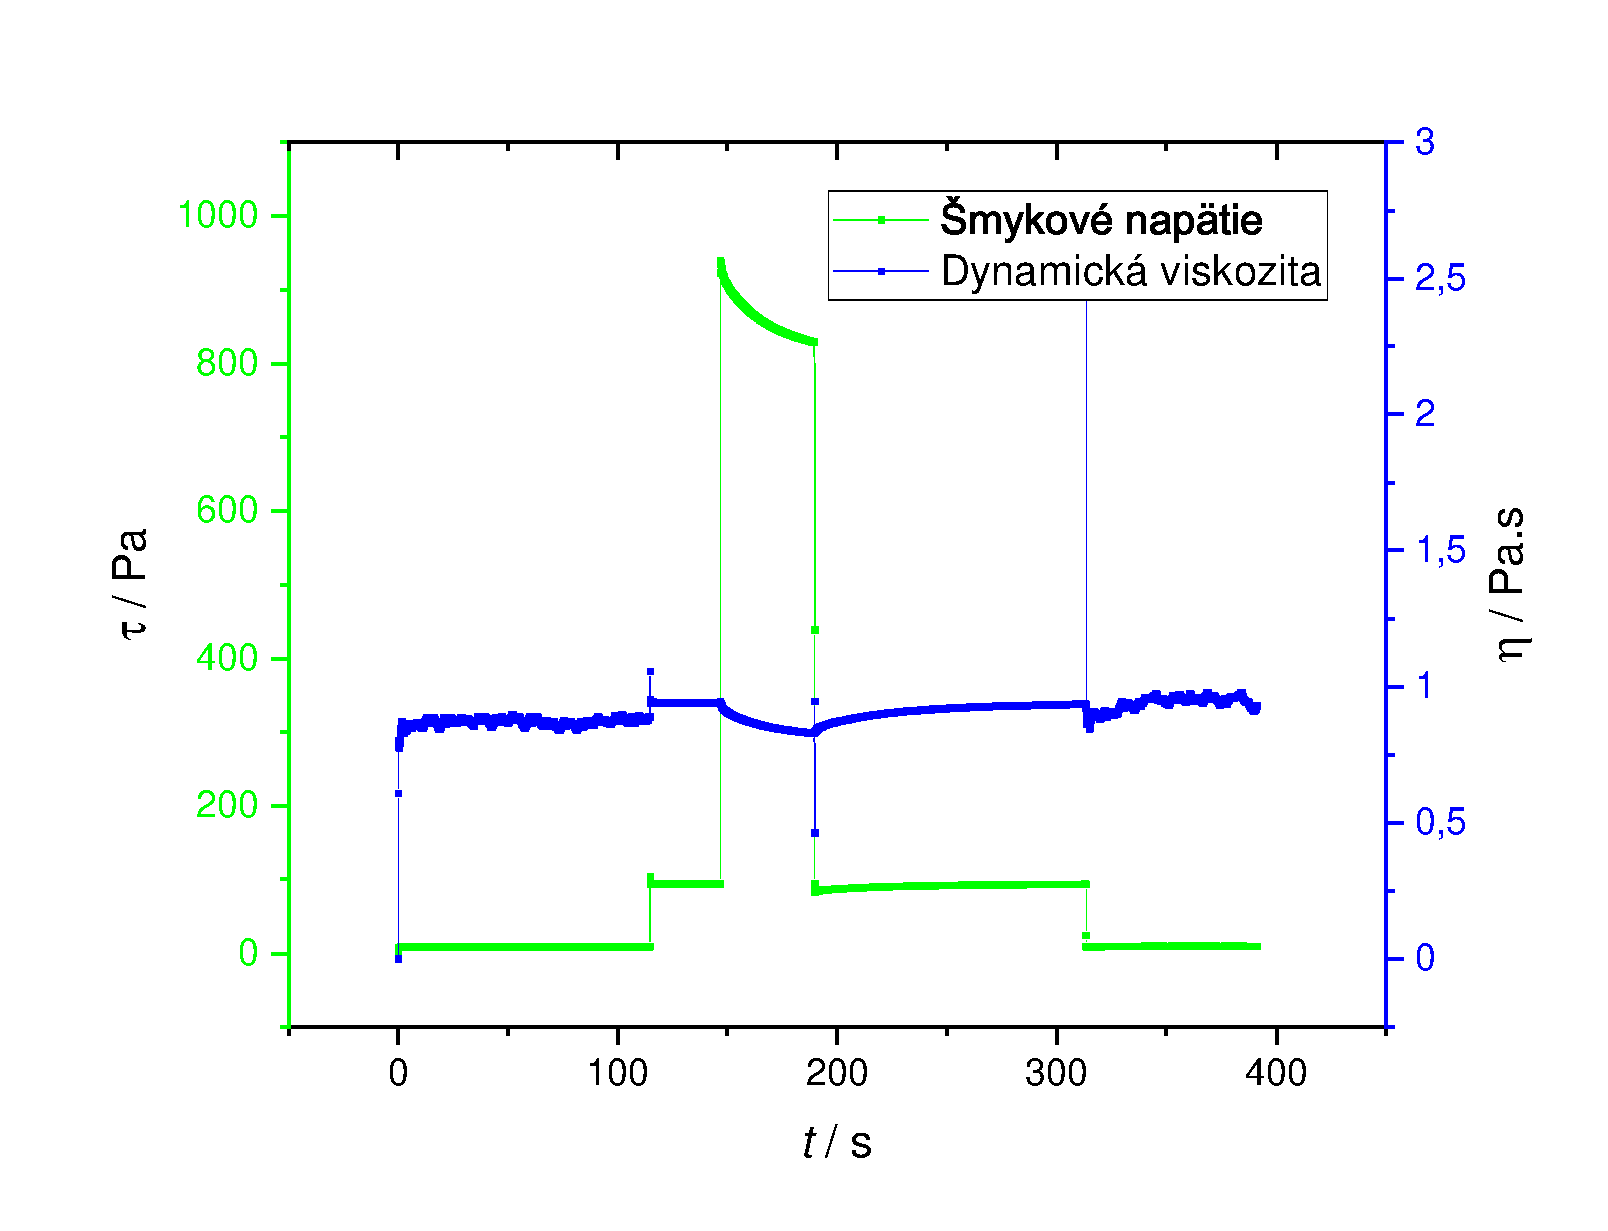
\includegraphics[width=0.8\textwidth]{GlycerinCas.pdf}
    \caption{Závislosť šmykového napätia a dynamickej viskozity od času pre glycerín}
    \label{fig:sub1}
\end{figure}

\emph{Poznámka ku grafu:} V tomto grafe boli nastavené rôzne rýchlosti šmykovej deformácie. 
To, kde sme menili hodnotu rýchlosti šmykovej deformácie si môžeme všimnúť pri náhlej zmene hodnôt šmykového napätia. 
V prvom úseku je rýchlosť šmykovej deformácie rovná $10~\mathrm{s}^{-1}$, v druhom úseku je rýchlosť šmykovej deformácie rovná $100~\mathrm{s}^{-1}$, v treťom úseku je rýchlosť šmykovej deformácie rovná $1000~\mathrm{s}^{-1}$, v štvrtom úseku je rýchlosť šmykovej deformácie rovná $100~\mathrm{s}^{-1}$ a v piatom úseku je rýchlosť šmykovej deformácie rovná $10~\mathrm{s}^{-1}$. 
Na rozhraní týchto rozdielnych rýchlostí šmykovej deformácie máme masívne výkyvy dynamickej viskozity, no tie sú spôsobené iba oneskorením záznamu dát a nenosia v sebe fyzikálny význam, čiže ich môžeme zanedbávať.\\

Ako sme povedali v postupe merania, tak chybu určenia viskozity sme odhadli pri štatistickom spracovaní hodnôt dynamickej viskozity pri rýchlosti šmykovej deformácie $10~\mathrm{s}^{-1}$. 
Toto spracovanie sme urobili tak, že sme zobrali veľkú väčšinu hodnôt dynamickej viskozity a pomocou programu \textbf{Excel} sme našli ich priemernú hodnotu a maximálnu a minimálnu hodnotu. 
Ako chybu určenia dynamickej viskozity sme určili väčšiu hodnotu medzi absolútnym rozdielom priemernej hodnoty a minimálnej hodnoty, a medzi absolútnym rozdielom priemernej hodnoty a maximálnej hodnoty.
Pri tomto spracovaní sme nebrali do úvahy niekoľko krajných hodnôt, nech predídeme chybe kvôli oneskoreniu merania hodnôt. No kvôli tomu sme mohli aj stratiť niektoré vhodné hodnoty a preto hovoríme o odhade chyby napriek tomu, že sme ich štatisticky spracovali.

Touto metódou sme získali chybu určenia dynamickej viskozity ako $u_{\eta}= 50~\mathrm{mPa.s}$.\\

Túto hodnotu sme určili prí rýchlosti šmykovej deformácie $10~\mathrm{s}^{-1}$, pretože u tejto rýchlosti amplitúdy výkyvov prevyšovali amplitúdy výkyvov pri rýchlosti šmykovej deformácie $100~\mathrm{s}^{-1}$ po ustálení. 
Rýchlosť šmykovej deformácie $1000~\mathrm{s}^{-1}$ sme neuvažovali, pretože toto meranie už nie je presné, kvôli tomu, že sa glycerín pri takej rýchlosti začne otepľovať, čo bude spôsobovať pokles dynamickej viskozity v priebehu času, ako si môžeme všimnúť v grafe \ref{fig:sub1}.\\

Následne sme zmerali tokové krivky pre glycerín pri teplotách $20~^\circ \mathrm{C}$ a $30~^\circ \mathrm{C}$. 
Tieto krivky sú obsiahnuté v grafoch \ref{fig:sub2} a \ref{fig:sub3}.

\begin{figure}[H]
\centering
\begin{subfigure}[t]{0.65\textwidth}  % zmena šírky z 0.48 na 0.95
\centering
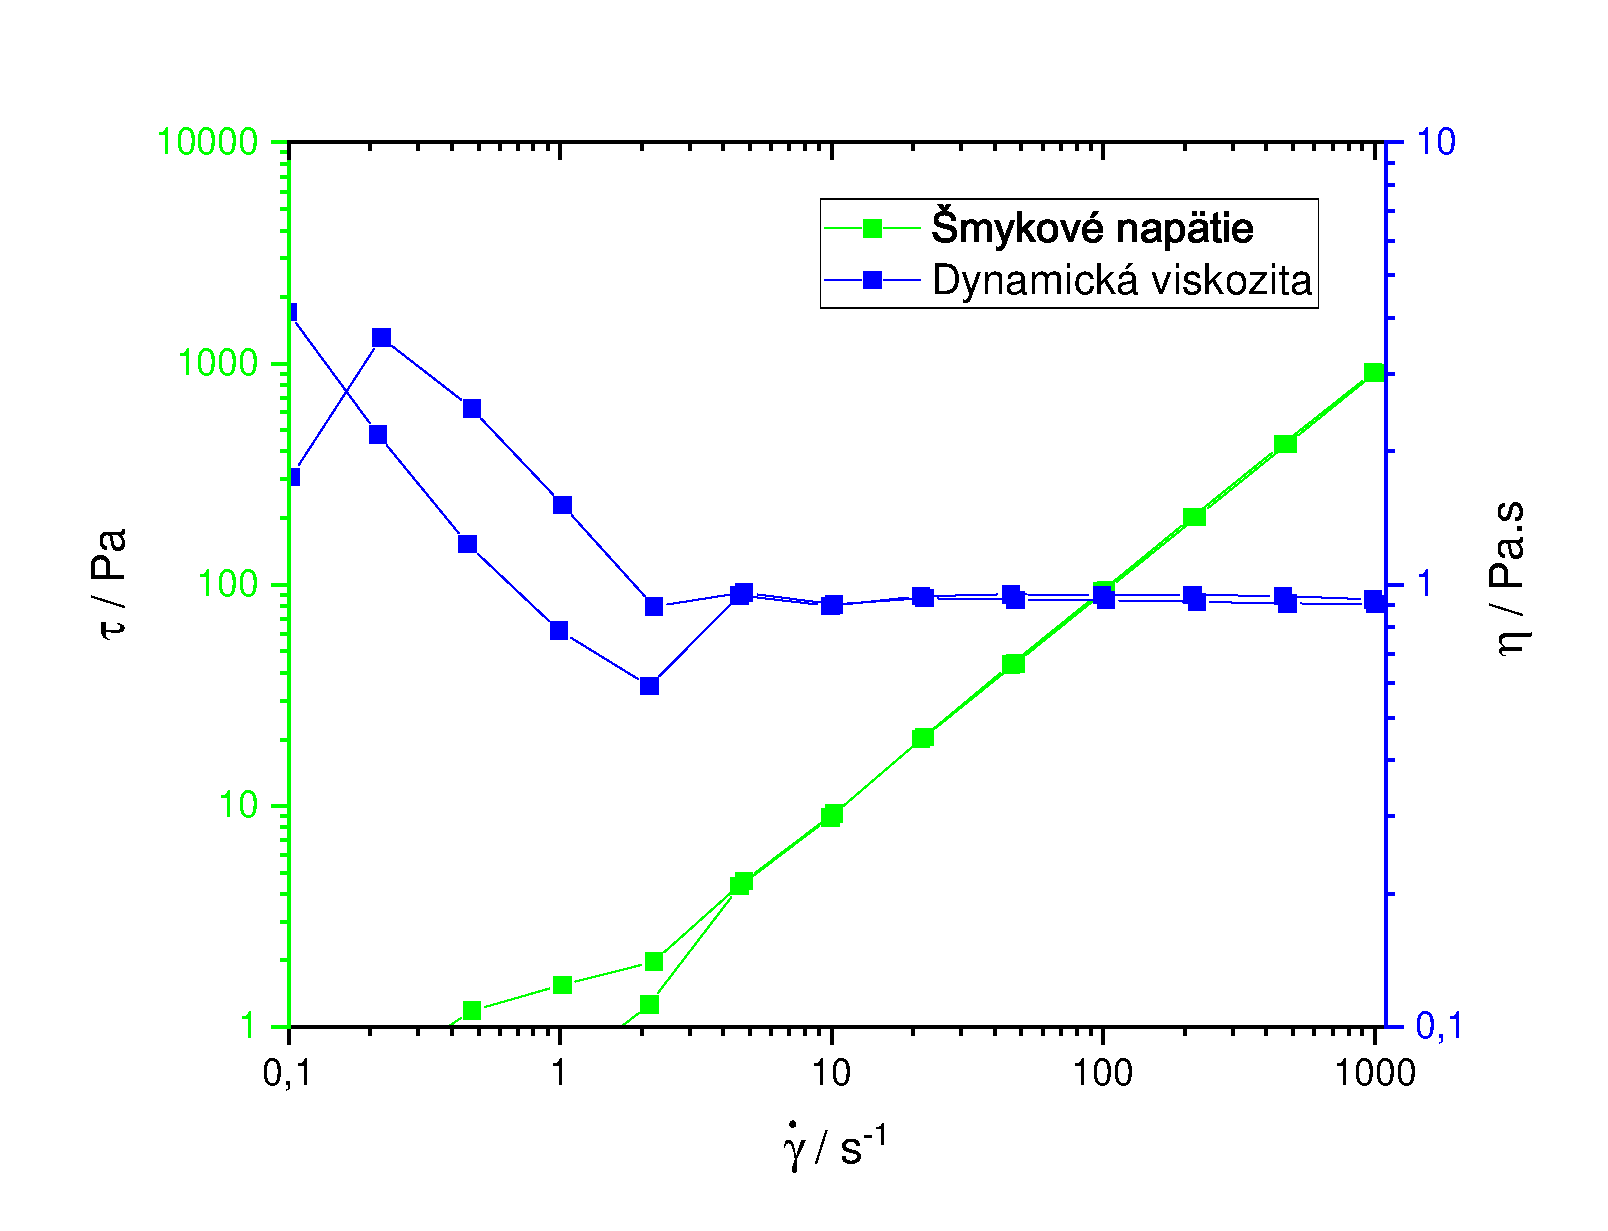
\includegraphics[width=\linewidth]{Glycerin20C.pdf}
\caption{Toková krivka glycerínu pri teplote $20~^\circ \mathrm{C}$}
\label{fig:sub2}
\end{subfigure}

\vspace{1cm}  

\begin{subfigure}[t]{0.65\textwidth}  % zmena šírky z 0.48 na 0.95
\centering
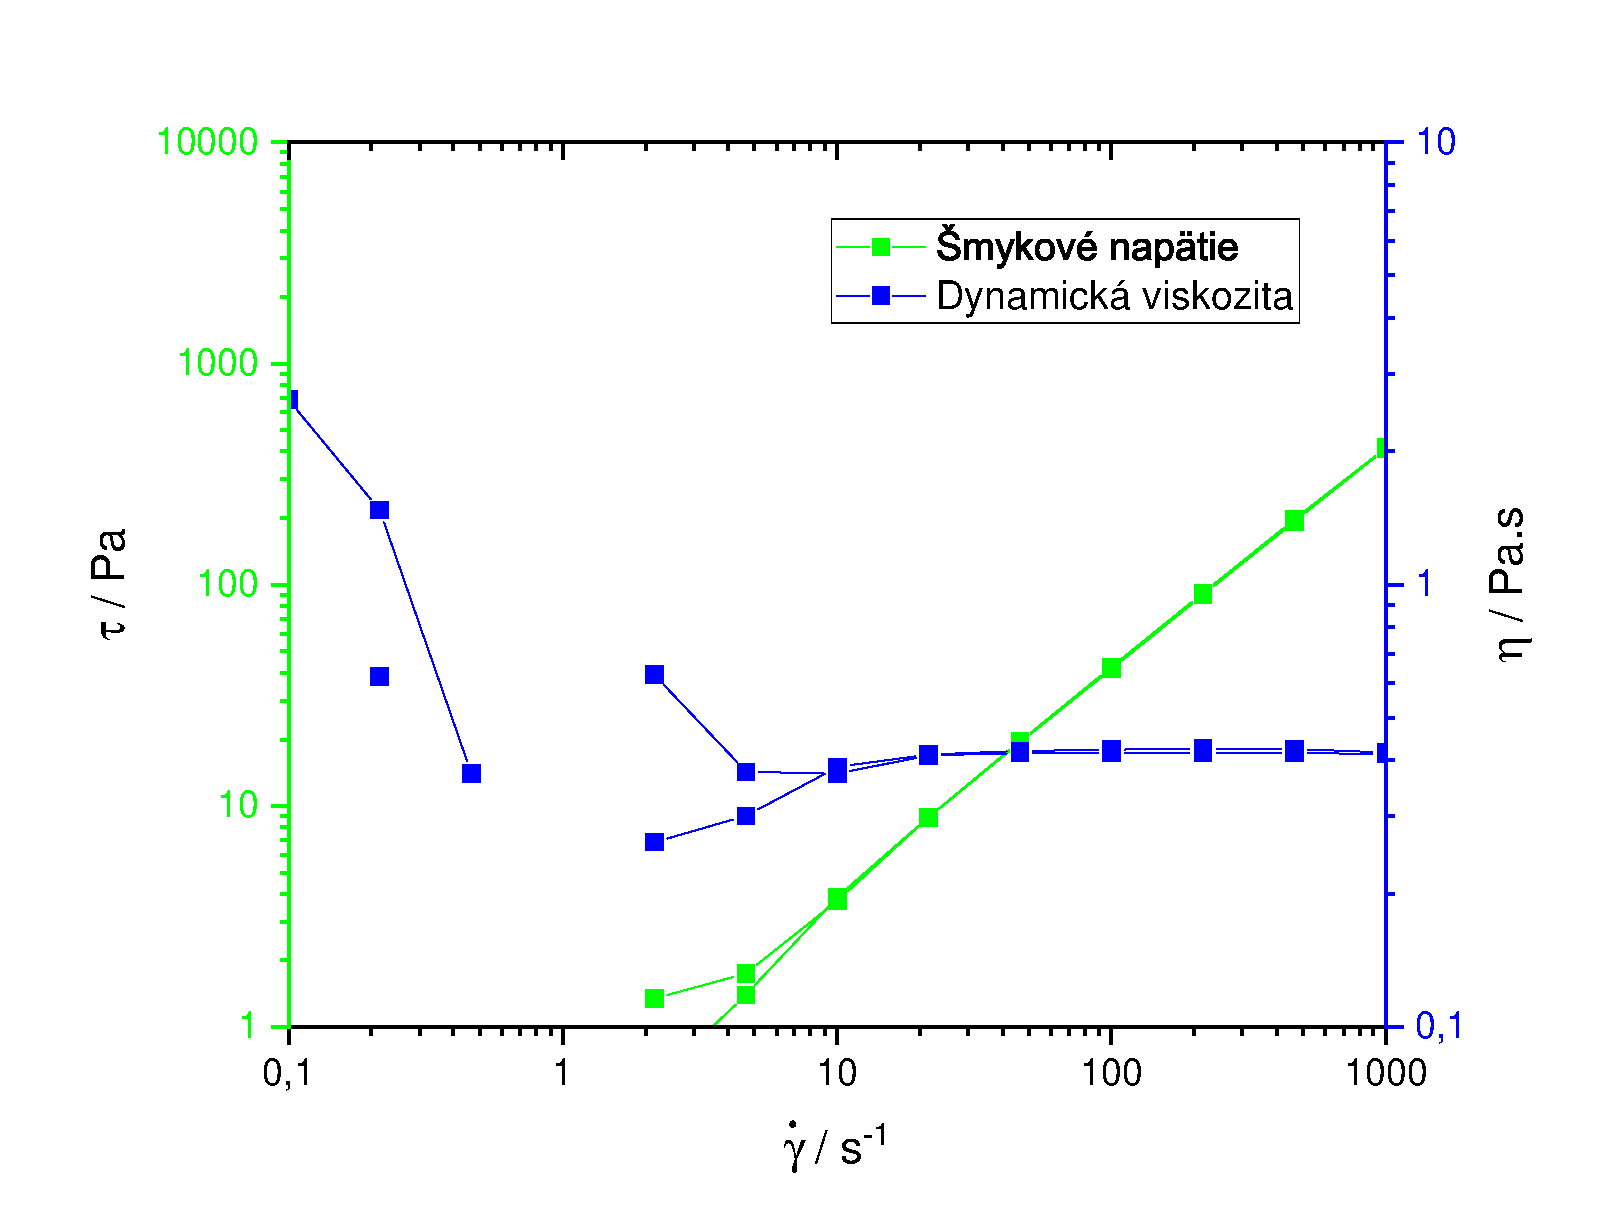
\includegraphics[width=\linewidth]{Glycerin30C.pdf}
\caption{Toková krivka glycerínu pri teplote $30~^\circ \mathrm{C}$}
\label{fig:sub3}
\end{subfigure}
\caption{Tokové krivky glycerínu pri rôznych teplotách}
\label{fig:both}
\end{figure}
\vspace{1cm}

\emph{Poznámka ku grafom:} Ako sme popísali v postupe merania, tak tieto grafy sú v log--log škálach. 
Môžeme si všimnúť, že v ľavej časti týchto grafov sa krivky nesprávajú podľa našich teoretických predpokladov a to je spôsobené nízkou rýchlosťou deformácie. 
Toto môže byť zapríčinené buď nedostatočným šmykovým tokom, ktorý by spôsobil nepresnosti v meraní, alebo tým, že sa nachádzame v dolnom rozsahu prístroja.
Preto budeme uvažovať iba pravú časť grafu, kde sa naše hodnoty chovajú podľa teoretických predpokladov, čiže približne od rýchlosti šmykovej deformácie $10~\mathrm{s}^{-1}$. 
Takisto si môžeme všimnúť, že že pre každú závislosť máme dve krivky a to je zapríčinené tým, že najprv sme rýchlosť šmykovej deformácie zrýchľovali a potom spomaľovali.

\subsection*{Určenie aktivačnej energie a teplotná závislosť dynamickej viskozity glycerínu}

Počas merania závislosti dynamickej viskozity na teplote sme najprv nastavili lineárny ohrev vzorku z $10~^\circ \mathrm{C}$ až po $40~^\circ \mathrm{C}$ a potom ho začali ochladzovať späť na $10~^\circ \mathrm{C}$. 
Toto meranie sme urobili pri konštantnej rýchlosti šmykovej deformácie $10~\mathrm{s}^{-1}$. 
Táto závislosť je obsiahnutá v grafe \ref{fig:Teplo}.

\begin{figure}[H]
    \centering
    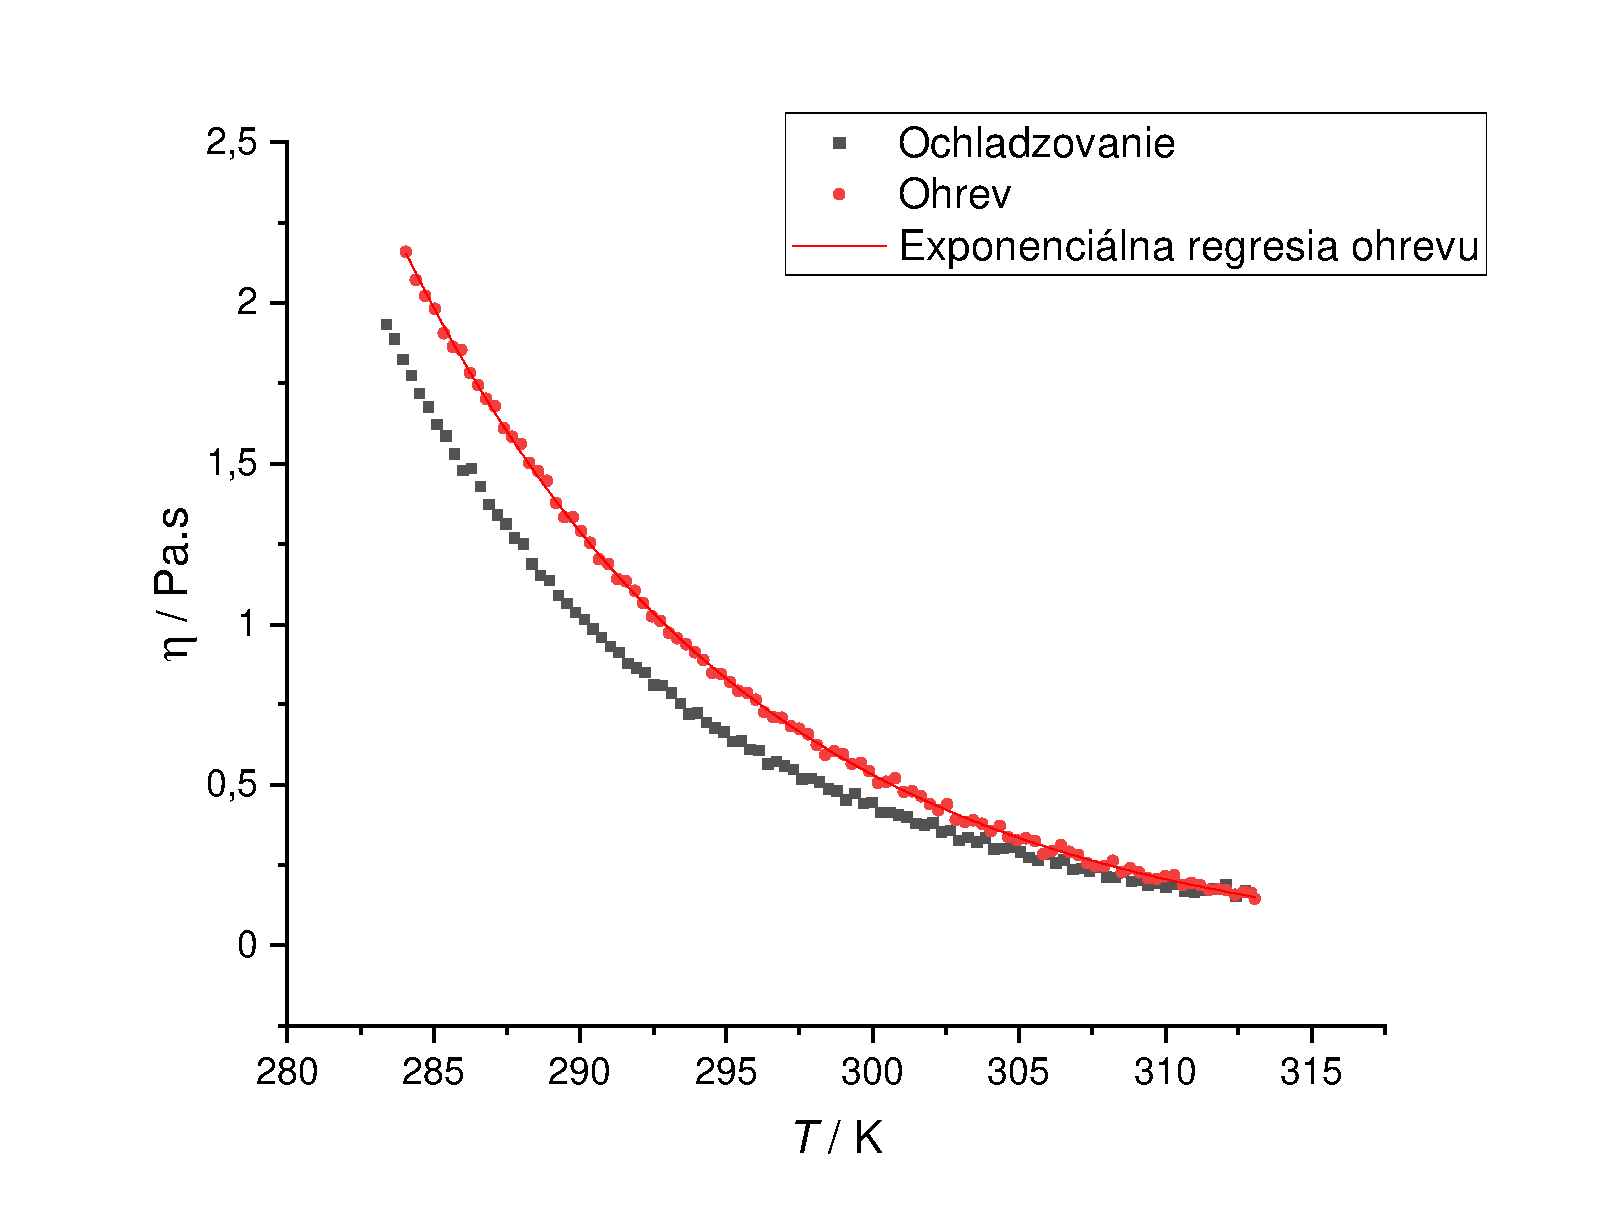
\includegraphics[width=0.8\textwidth]{TeplotnaZavislosť.pdf}
    \caption{Závislosť dynamickej viskozity od termodynamickej teploty}
    \label{fig:Teplo}
\end{figure}

\emph{Poznámka ku grafu:} V tomto grafe sme previedli teplotu, ktorá bola nameraná v stupnici Celzia do termodynamickej stupnice. 
Môžeme si všimnúť, že krivka pri ochladzovaní neodpovedá krivke pri ohreve. To je spôsobené hysteréziou. 
Preto na určenie aktivačnej energie $\varepsilon_A$ budeme uvažovať exponenciálnu regresiu ohrevu systému, keďže ten sme robili prvý a nie je ešte zaťažený hysteréziou. 
Túto exponenciálnu regresiu sme urobili pomocou programu \textbf{Origin}, ktorý ju urobil metódou najmenších štvorcov. 
Chybové úsečky sa v tomto grafe nachádzajú, no vzhľadom na rozsah oboch osí sú príliš malé aby boli pozorovateľné.\\

Tento graf sa nám chová podľa závislosti \ref{eq:TeplotnaZavislost}, avšak s tým, že v závislosti \ref{eq:TeplotnaZavislost} je termodynamická teplota v menovateli a program \textbf{Origin} nám vyhodnotí exponenciálnu regresiu podľa vzťahu $y=y_0 + A\mathrm{exp}(Bx)$. 
Čiže nato, aby sme správne vedeli z $B$ vyvodiť aktivačnú energiu, tak potrebujeme urobiť graf, kde na x--ovej osi bude prevrátená hodnota termodynamickej teploty. 
Takáto závislosť je obsiahnutá v grafe \ref{fig:Prevratena}.


\begin{figure}[H]
    \centering
    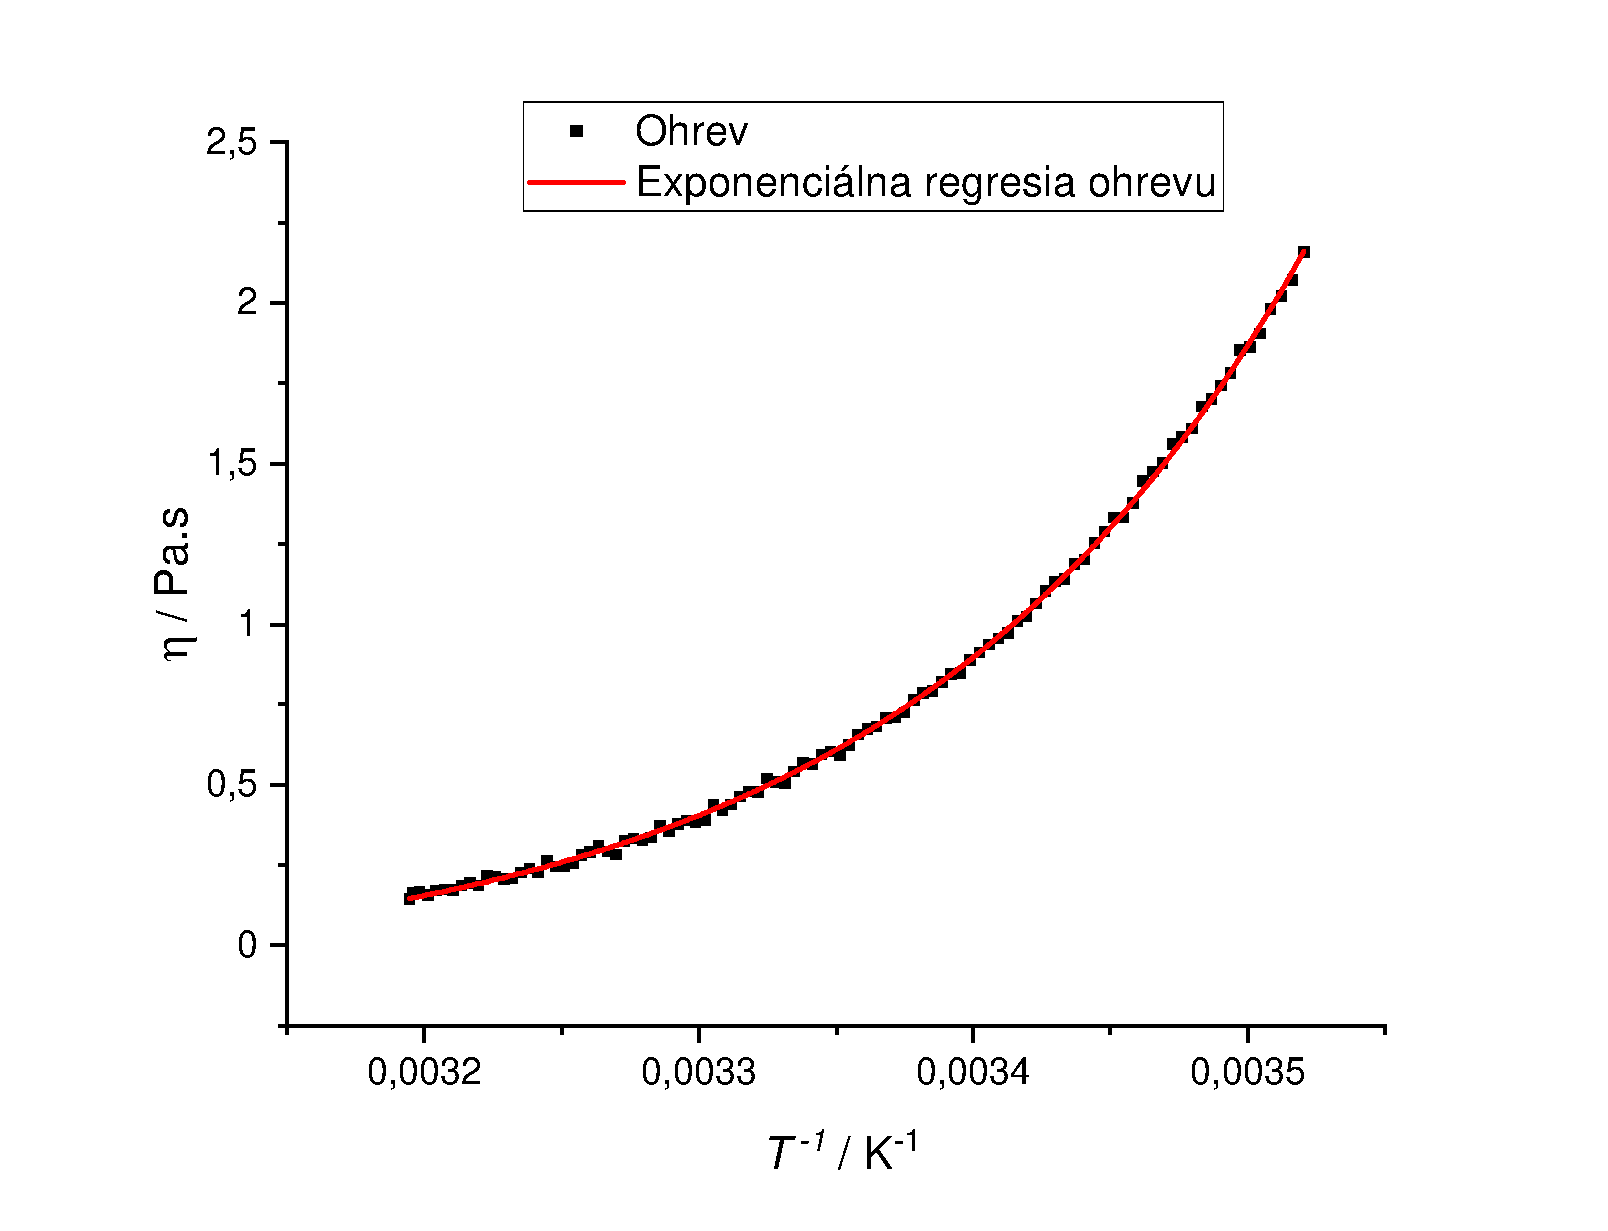
\includegraphics[width=0.8\textwidth]{Prevratena.pdf}
    \caption{Závislosť dynamickej viskozity od prevrátenej hodnoty termodynamickej teploty}
    \label{fig:Prevratena}
\end{figure}

Program \textbf{Origin} nám teda pomocou metódy najmenších štvorcov vyhodnotil exponenciálnu regresiu
$y=y_0 + A\mathrm{exp}(Bx)$, pričom $y_0$ zodpovedá hodnote posunu, po anglicky offsetu, ktorá nie je uvažovaná v teoretickom modeli a keďže nám vychádza jej hodnota veľmi malá, tak ju ani mi nebudeme uvažovať. 
$A$ zodpovedá konštante $C$ a $B$ zodpovedá hodnote $\frac{\varepsilon_A}{k}$, čiže práve tento parameter  $B$ exponenciálnej regresie pre nás bude kľúčový.
Program \textbf{Origin} nám pri vykonaní exponenciálnej regresie vyhodnotil štatistickú chybu parametrov, v ktorej sú zahrnuté chybové úsečky určenia teploty a dynamickej viskozity, kde tieto neistoty sme popísali vyššie.

Program \textbf{Origin} nám teda vyhodnotil exponenciálnu regresiu:

\[
\eta =y_0+A\mathrm{exp}(\frac{B}{T}),
\]

kde $y_0 = -0,10(1)$, $A = 9(2)\times10^{-11}$ a $B = 6790(50)$.\\

Keďže $B = \frac{\varepsilon_A}{k}$, tak aktivačnú energiu $\varepsilon_A$ vypočítame podľa vzťahu

\begin{equation}
		\varepsilon_A = Bk.
		\label{eq:Energia}
\end{equation} \\


Boltzmannova konštanta je podľa \cite{MatFyzTabulky} rovná $k=1,38054(18)\times10^{-23}~\mathrm{JK}^{-1}$. 
Avšak neistotu určenia Boltzmannovej konštanty nebudeme uvažovať, pretože je rádovo nižšia než ostatné neistoty. Neistotu určenia aktivačnej energie $u_{\varepsilon_A}$ teda určíme ako 

\begin{equation}
		u_{\varepsilon_A} = u_Bk,
		\label{eq:ChybaEnergia}
\end{equation} \\

kde $u_B$ je štatistická chyba určenia parametru $B$ exponenciálnej regresie.\\

Zo vzťahov \ref{eq:Energia} a \ref{eq:ChybaEnergia} sme vypočítali $\varepsilon_A$ ako 

\[
\varepsilon_A = 9,37(7)\times10^{-20}~\mathrm{J}.
\]\\

\subsection*{Meranie tokových kriviek pre škrob}

Najprv sme rovnakým spôsobom, ako sme robili pre glycerín, dali do rotačného viskozimetra škrob a potom sme merali časovú závislosť dynamickej viskozity a šmykového napätia pre rôzne rýchlosti šmykovej deformácie pri pokojovej teplote, ktorú uvažujeme na $24~^\circ \mathrm{C}$. 
Je pravda, že počiatočnú pokojovú teplotu  sme namerali na $24,3(1)~^\circ \mathrm{C}$, no tento rozdiel teplôt sa nám minimálne prejaví v meraní rozsahu rýchlosti šmykovej deformácie a preto ho nebudeme uvažovať.\\

V programe \textbf{HAAKE RheoWin Job Manager} sme nastavili, nech nám počas merania závislosti dynamickej viskozity a šmykovej deformácie od času vyhodnocuje tieto údaje v skokovom grafe. 
Tieto dáta sme vyhodnotili v programe \textbf{Origin}, kde y--osi sú v logaritmických škálach kvôli lepšej prehľadnosti. 
Počas merania sme menili rýchlosť šmykovej deformácie, čo sa prejavilo v skokoch grafu. 
Táto závislosť je obsiahnutá v grafe \ref{fig:SkrobCas}.

\begin{figure}[H]
    \centering
    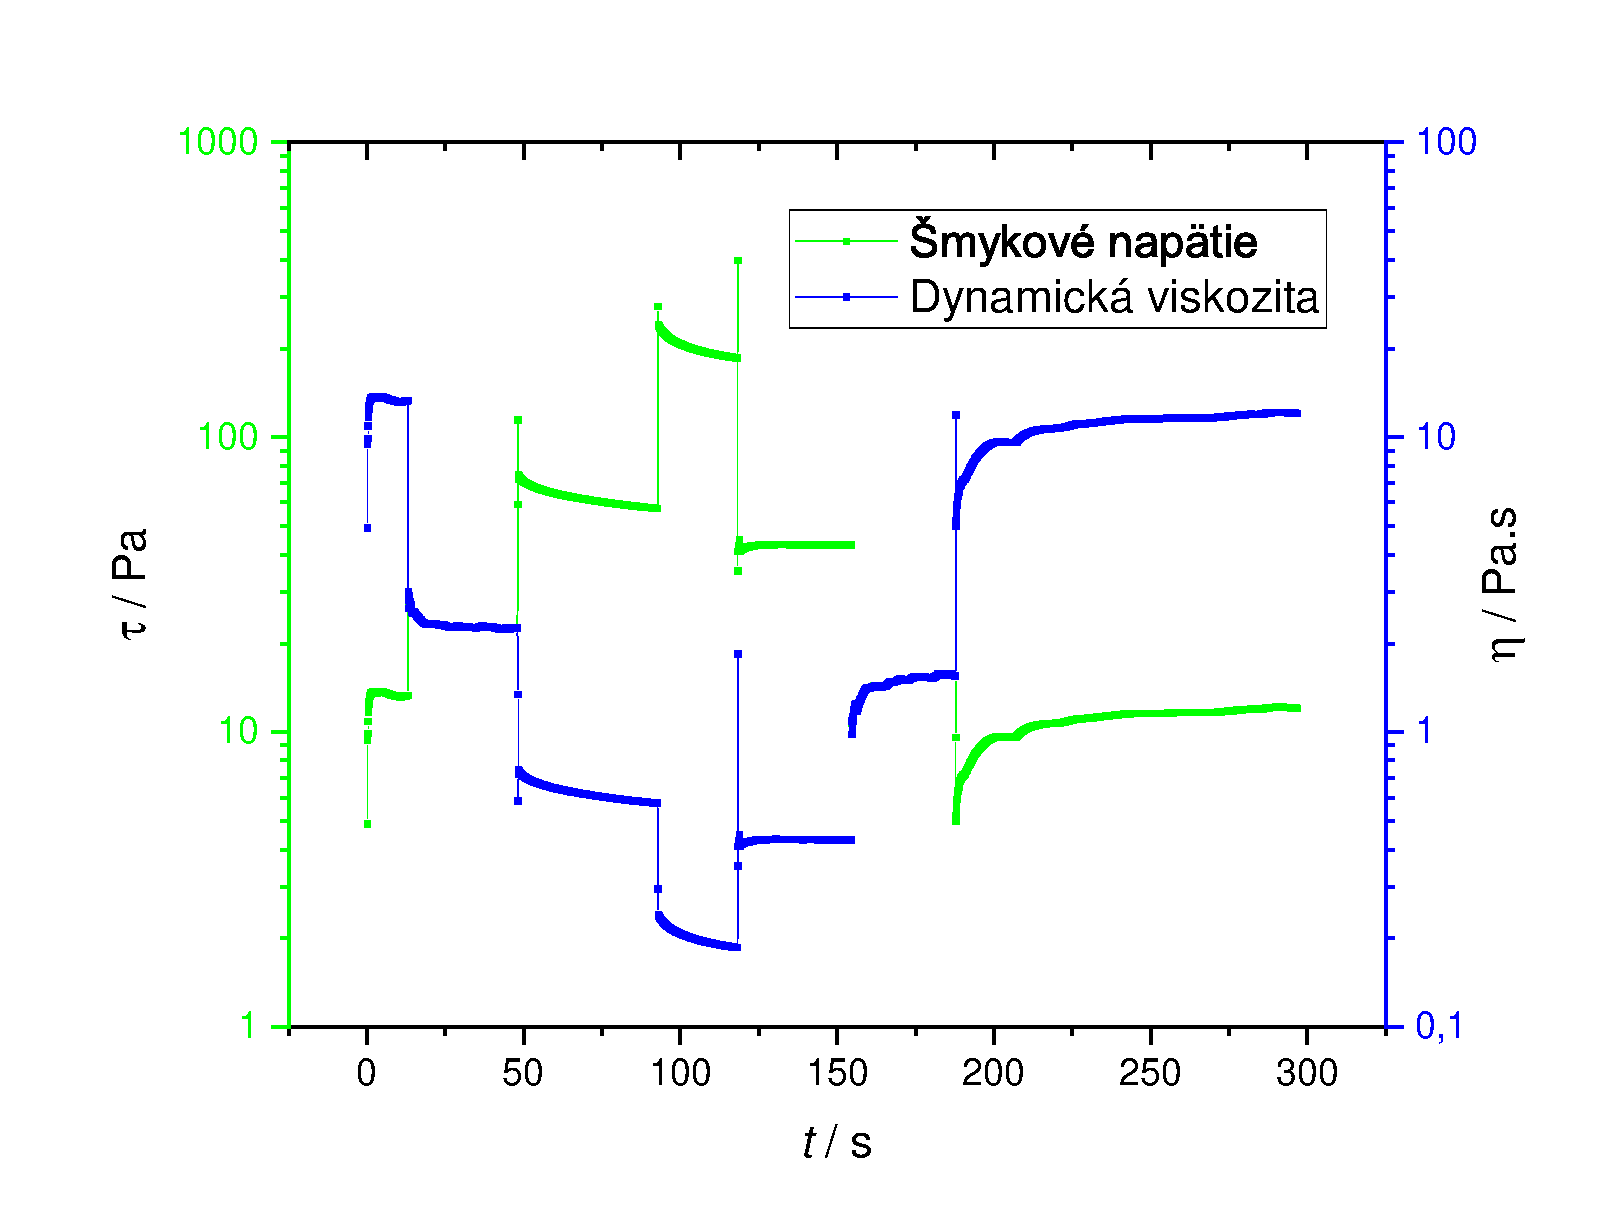
\includegraphics[width=0.8\textwidth]{SkrobCas.pdf}
    \caption{Závislosť šmykového napätia a dynamickej viskozity od času pre škrob}
    \label{fig:SkrobCas}
\end{figure}

\emph{Poznámka ku grafu:} V tomto grafe sa zmeny rýchlosti prejavujú výraznými skokmi dynamickej viskozity a šmykového napätia. 
V prvom úseku je rýchlosť šmykovej deformácie rovná $1~\mathrm{s}^{-1}$, v druhom úseku je rýchlosť šmykovej deformácie rovná $10~\mathrm{s}^{-1}$, v treťom úseku je rýchlosť šmykovej deformácie rovná $100~\mathrm{s}^{-1}$, v štvrtom úseku je rýchlosť šmykovej deformácie rovná $1000~\mathrm{s}^{-1}$, v piatom úseku je rýchlosť šmykovej deformácie opäť rovná $100~\mathrm{s}^{-1}$, v šiestom úseku je rýchlosť šmykovej deformácie rovná $10~\mathrm{s}^{-1}$ a v siedmom úseku je rýchlosť šmykovej deformácie rovná $1~\mathrm{s}^{-1}$.
Podobne ako pri grafe \ref{fig:sub1} pre glycerín si môžeme všimnúť abnormálne skoky hodnôt na rozhraní zmien rýchlostí šmykovej deformácie, no tie sú tiež spôsobené oneskorením záznamu dát, čiže nemajú fyzikálny význam a naďalej ich neuvažujeme. 
Môžeme si takisto všimnúť, že pre rýchlosť šmykovej deformácie $10~\mathrm{s}^{-1}$ krivka šmykového napätia a dynamickej viskozity splývajú.  \\

Môžeme si všimnúť, že keď navraciame hodnoty rýchlostí šmykovej deformácie, tak hodnoty dynamickej viskozity a šmykového napätia sú iné ako keď sme ich pôvodne mali danú rýchlosť šmykovej deformácie. 
Toto je takisto spôsobené hysteréziou systému, ako sme predpokladali v teórii a preto budeme uvažovať iba časti, kde sme zvyšovali rýchlosť šmykovej deformácie. 
Predpokladáme, že škrob je nenewtonovská látka, pre ktorú je typické, že so zvyšujúcou sa rýchlosťou šmykovej deformácie sa dynamická viskozita znižuje.
Keď sa pozrieme na jednotlivé úseky, tak si môžeme všimnúť že v oblasti s rýchlosťou šmykovej deformácie $1~\mathrm{s}^{-1}$ krivka stúpa a až od nejakého bodu začne klesať ako by sme predpokladali, to je nekonzistentné s našou teóriou preto túto rýchlosť šmykovej deformácie vylúčime z rozsahu merania. 
Pri rýchlostiach šmykových deformácii $10~\mathrm{s}^{-1}$ a $100~\mathrm{s}^{-1}$ sa krivky chovajú podľa našich očakávaní, čiže tie budeme brať do našeho rozsahu. 
A u rýchlosti šmykovej deformácie $1000~\mathrm{s}^{-1}$ sa krivky tiež správajú podľa našich predpokladov, čiže túto rýchlosť budeme tiež uznávať do rozsahu, avšak môžeme si všimnúť že krivky klesajú pomerne výraznejšie než u ostatných oblastí, čo môže naznačovať že sa blížime k hornej hranici rozsahu, kde sa narúša štruktúra škrobu a môže dôjsť k nestabilite toku.\\

Z vyššie uvedených úvah označíme rozsah použiteľnej rýchlosti šmykovej deformácie ako $\langle 10~\mathrm{s}^{-1}, 1000~\mathrm{s}^{-1}\rangle$.\\


Následne sme namerali tokovú krivku škrobu. V nej sme postupne menili rýchlosť šmykovej deformácie, pričom sme jednu chvíľu merali aj v okolí $1~\mathrm{s}^{-1}$, nech si môžeme všimnúť ako sa tam bude krivka správať. 
Táto toková krivka škrobu je obsiahnutá v grafe \ref{fig:SkrobTok}. 

\begin{figure}[H]
    \centering
    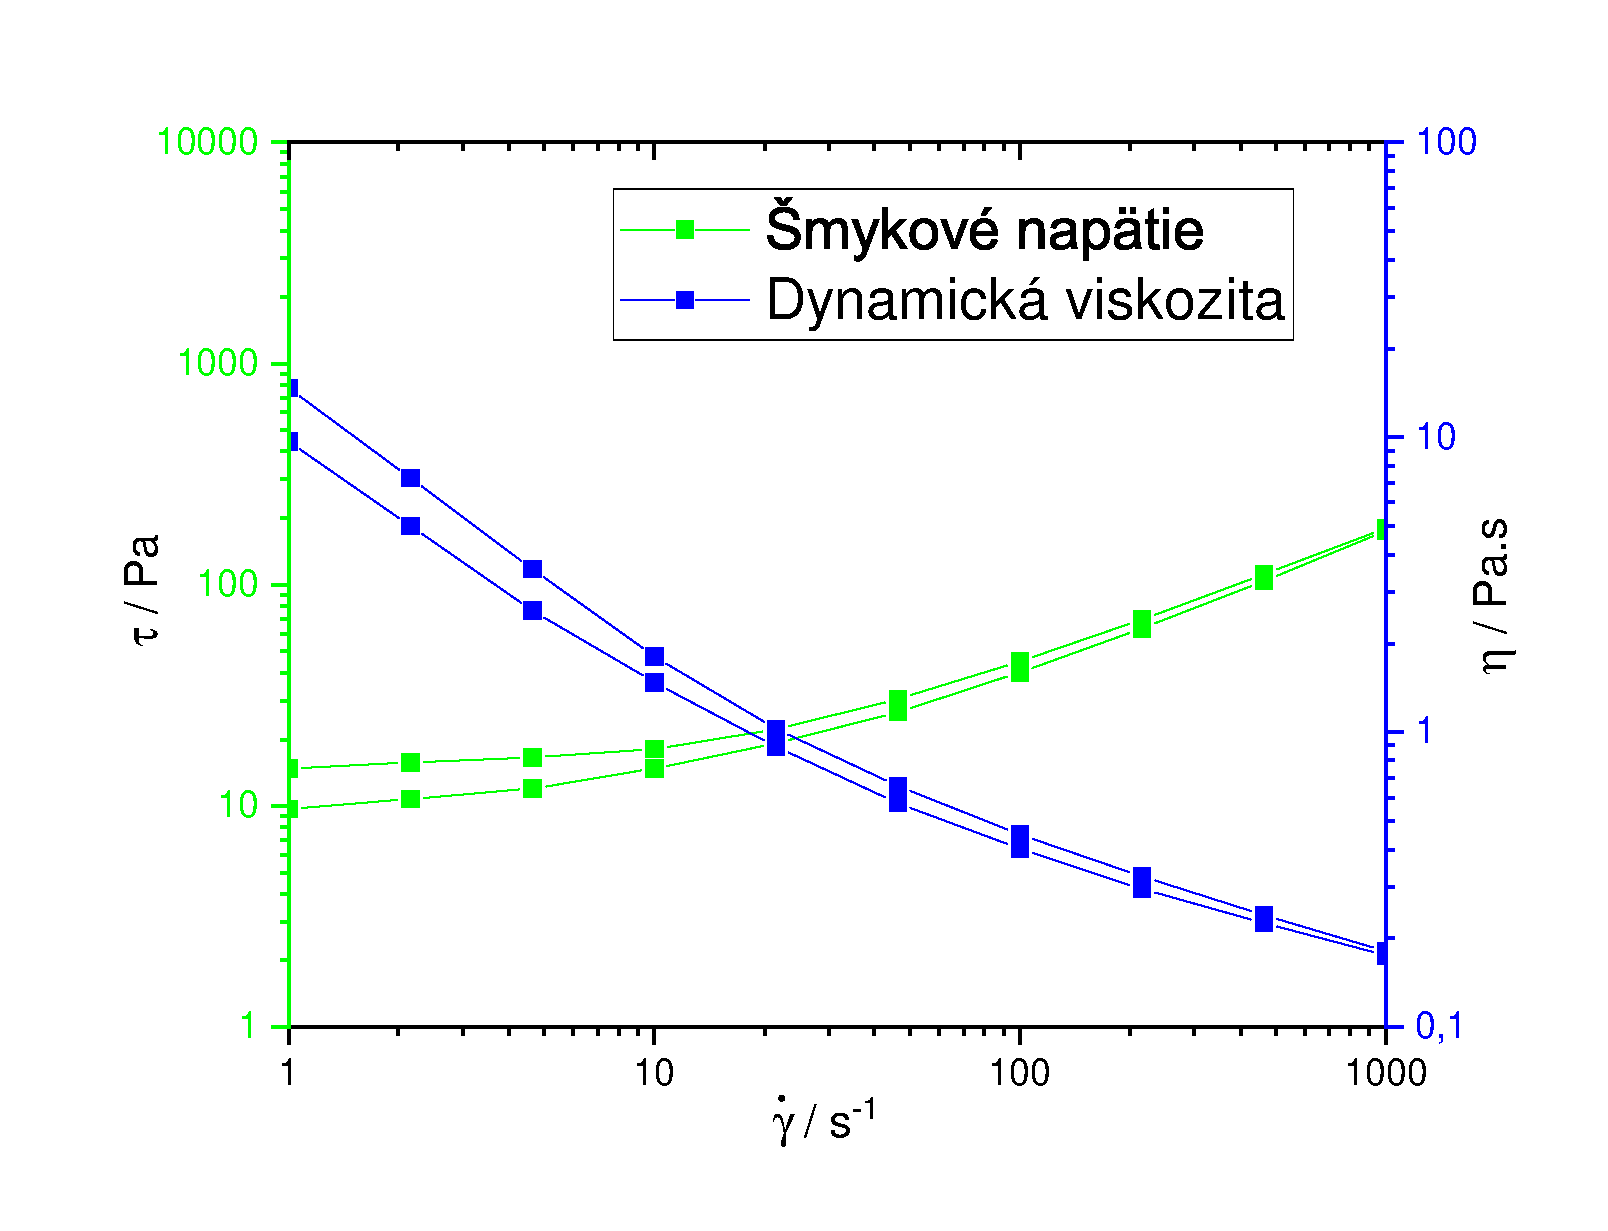
\includegraphics[width=0.8\textwidth]{SkrobRovnicaToku.pdf}
    \caption{Toková krivka škrobu}
    \label{fig:SkrobTok}
\end{figure}

\emph{Poznámka ku grafu:} Tento graf je v log--log škále kvôli lepšej prehľadnosti. 
Môžeme si všimnúť celkom zvláštne správanie, že krivky sa pri znižovaní rýchlosti šmykovej deformácie výrazne odlišujú od pôvodných hodnôt, avšak toto je konzistentné s našou teóriou, kde sme povedali, že reologické správanie škrobu je zaťažené hysteréziou, ktorá sa nám prejavila v tomto grafe. 

\subsection*{Určenie hustoty a koncentrácie glycerínu}

Podľa postupu uvedeného v postupe merania sme pomocou digitálnych váh zmerali hmotnosť pyknometra aj s uzáverom $m_1$, hmotnosť pyknometra naplneného destilovanou vodou $m_2$ a hmotnosť pyknometra naplneného glycerínom $m_3$. 
Tieto hodnoty sú obsiahnuté v tabuľke \ref{tab:Pyknometer}.

\begin{table}[H]
    \centering
    \renewcommand{\arraystretch}{1.2}
    \caption{Meranie hmotností}
    \label{tab:Pyknometer}
    \adjustbox{max width=\textwidth}{
    \begin{tabular}{|c|c|}
        \hline  
    
         & $m$ / g \\
        \hline
        $m_1$  & 28,64(2)  \\
        $m_2$  & 53,40(2)  \\
        $m_3$ & 59,79(2)\\
        \hline
        
    \end{tabular}
    }
\end{table}


Je pravda, že neistota určenia hmotnosti pomocou digitálnych váh je $\pm~0,001~\mathrm{g}$, no kvôli tomu, že sme merali glycerín, ktorý sa veľmi ľahko prilepí na vrch pyknometra a nejde zmyť bude neistota merania hmotnosti digitálnych váh zanedbateľná oproti tejto neistote spôsobenej prilepeným glycerínom na pyknometri. 
Preto odhadneme neistotu určenia hmotnosti na $\pm~0,02~\mathrm{g}$.\\

Potom sme pri nameranej pokojovej teplote $24,3(1)~^\circ \mathrm{C}$ určili hustotu destilovanej vody ako $\rho_1 = 997,2~\mathrm{kg.m}^{-3}$ podľa \cite{MatFyzTabulky}.
Chybu určenia hustoty destilovanej vody považujeme za zanedbateľnú, keďže pri našej neistote určenia teploty by zmena hustoty bola zanedbateľná oproti ostatným chybám. 
Následne sme vypočítali hustotu glycerínu podľa vzťahu \ref{eq:Pyknometer}. 
Neistotu určenia hustoty glycerínu $u_{\rho_2}$ sme určili využitím štandardného prenosu neistôt vo vzorci \ref{eq:Pyknometer}, z čoho sme dostali vzorec


\begin{equation}
		u_{\rho_2} = \rho_2\sqrt{2}u_m\sqrt{\frac{1}{(m_3-m_1)^2}+\frac{1}{(m_2-m_1)^2}},
		\label{eq:ChybaHustota}
\end{equation} \\

kde $u_m$ je neistota určenia hmotnosti.\\

Hustotu glycerínu aj s jeho neistotou sme určili podľa vzorcov \ref{eq:ChybaHustota} a \ref{eq:Pyknometer} ako $\rho_2 = 1255(2)~\mathrm{kg.m}^{-3}$. 
Z tejto hodnoty sme pri preštudovaní tabuľkových hodnôt \cite{Koncentrácia} zistili, že táto hustota pri teplote $25~^\circ \mathrm{C}$ najviac vyhovuje koncentrácii 99\% glycerínu v roztoku vody s glycerínom. 
Podiel vody v roztoku glycerínu teda je 1\%.

\newpage
\section*{Diskusia výsledkov}

Pre glycerín sme zmerali závislosť dynamickej viskozity a šmykového napätia od času, pričom táto závislosť sa nachádza v grafe \ref{fig:sub1}. 
Môžeme si z neho všimnúť, že dynamická viskozita je približne konštantná, až na rýchlosť šmykovej deformácie $1000~\mathrm{s}^{-1}$, čo je pravdepodobne zapríčinené tým, že pri takejto vysokej rýchlosti šmykovej deformácie sa vzorka začala ohrievať čo spôsobovalo pokles dynamickej viskozity. 
Preto túto rýchlosť neuvažujeme. 
Avšak okrem tejto jednej rýchlosti šmykovej deformácie si môžeme všimnúť, že dynamická viskozita je približne konštantná, čo zodpovedá faktu, že glycerín je newtonovská kvapalina.\\

Náš odhad chyby určenia viskozity by mal byť presný kvôli tomu, že výkyvy dynamickej viskozity pri rýchlosti šmykovej deformácie $10~\mathrm{s}^{-1}$ sú najväčšie, čo znamená, že ak určíme najväčší výkyv pri takejto rýchlosti šmykovej deformácie, tak táto chyba bude pokrývať aj chyby pri ostatných rýchlostiach šmykových deformácii. 
Avšak takýmto spôsobom môžeme chybu nadhodnotiť a tomu by sme vedeli predísť tým, že by sme podrobnejšie štatisticky spracovali dáta a z toho určili priemernú hodnotu chyby určenia dynamickej viskozity.\\

Tokové krivky pre glycerín sme namerali pri teplotách $20~^\circ \mathrm{C}$ a $30~^\circ \mathrm{C}$. 
Tieto krivky sú obsiahnuté v grafoch \ref{fig:sub2} a \ref{fig:sub3}.
Môžeme si všimnúť, že v ľavej časti grafu sa krivky nechovajú podľa teoretických predpokladov, čo môže byť zapríčinené nedostatočným šmykovým tokom, aby ho prístroj s presnosťou meral ale takisto je pravdepodobné že tieto hodnoty sa nachádzajú v dolnom rozsahu merania prístroja.
Na to, aby sme zistili či sa rýchlosť šmykovej deformácie pri hodnote $1~\mathrm{s}^{-1}$ nachádza v použiteľnom rozsahu pre glycerín by sme museli urobiť znova závislosť dynamickej viskozity a šmykového napätia od času pri tejto rýchlosti šmykovej deformácie a pozorovať chovanie krivky pri tejto rýchlosti.\\

No pokiaľ budeme uvažovať iba pravú časť, približne od rýchlosti šmykovej deformácie $10~\mathrm{s}^{-1}$, tak tokové krivky zodpovedajú lineárnemu chovaniu newtonovskej látky, ktorou glycerín je. 
Takisto hodnoty dynamickej viskozity sú konštantné, čo tiež zodpovedá newtonovskému chovaniu glycerínu.
Pokiaľ porovnáme tieto tokové krivky, tak si môžeme všimnúť, že pri vyššej rýchlosti šmykovej deformácie je hodnota dynamickej viskozity nižšia, čo je konzistentné s našimi teoretickými predpokladmi.\\

Teplotnú závislosť dynamickej viskozity sme namerali v teplotnom rozsahu $10~^\circ \mathrm{C}$ až $40~^\circ \mathrm{C}$ a táto závislosť je obsiahnutá v grafe \ref{fig:Teplo}. 
Môžeme si všimnúť, že tento graf sa chová exponenciálne s prevrátenou hodnotou $T$ v exponente, čo je konzistentné so vzorcom \ref{eq:TeplotnaZavislost}, ktorý túto závislosť popisuje. 
Počas tohoto merania sme najprv ohrievali vzorku a potom ochladzovali a pri ochladzovaní bolo naše meranie zaťažené hysterézou systému. 
Toto mohlo byť zapríčinené nepresnou reguláciou teploty alebo príliš rýchlou zmenou teploty systému. 
Tejto hysteréze by sme mohli predísť tak, že by sme spomalili rýchlosť ohrevu, avšak to je časovo nevýhodné a takisto bezvýznamné, keďže k vyhodnoteniu aktivačnej energie nám stačí zobrať krivku ohrevu, ktorá nie je zaťažená hysterézou systému.\\

Aktivačnú energiu sme určili pomocou parametrov exponenciálnej regresie krivky \ref{fig:Prevratena}, ktorú nám vykonal program \textbf{Origin}, ako $\varepsilon_A = 9,37(7)\times10^{-20}~\mathrm{J}$. 
Neistotu určenia aktivačnej energie by sme mohli znížiť podrobnejším meraním teplotnej závislosti pre viac hodnôt, avšak to by bolo vysoko neefektívne vzhľadom k tomu, ako málo by sme zvýšili presnosť merania.\\

Rozsah použiteľnej rýchlosti šmykovej deformácie pre škrob sme určili ako $\langle 10~\mathrm{s}^{-1}, 1000~\mathrm{s}^{-1}\rangle$, pričom tieto hodnoty sme získali analýzou grafu \ref{fig:SkrobCas} pri pokojovej teplote $24~^\circ \mathrm{C}$. 
Tento rozsah je takisto konzistentný s rozsahom rýchlosti šmykovej deformácie škrobu, ktorý bol uvedený pri podobnom meraní v článku \cite{Skrob}. 
Avšak tento rozsah by sme mohli spresniť tak, že by sme sledovali chovanie krivky pri viacerých hodnotách rýchlostí šmykovej deformácie a pri ich sledovaní by sme zistili, kedy sa krivky nechovajú podľa teoretických predpokladov a z toho by sme určili aký je presnejší rozsah. 
Z grafu \ref{fig:SkrobCas} môžeme ešte podotknúť, že pre hodnoty rýchlostí šmykovej deformácie, ktoré sú v nami určenom rozsahu, dynamické viskozity nie sú konštantné, čo je charakteristické pre nenewtonovské látky a ukazuje že škrob je skutočne nenewtonovská látka.\\

Tokovú krivku pre škrob sme namerali pri teplote $24~^\circ \mathrm{C}$, ktorá bola blízka pokojovej teplote. 
Vzhľadom k nami predom zvolenému rozsahu uvažujeme iba časť tohoto grafu, počínajúceho od rýchlosti šmykovej deformácie $10~\mathrm{s}^{-1}$. 
Táto toková krivka je obsiahnutá v grafe \ref{fig:SkrobTok}. 
Môžeme si všimnúť, že toková krivka nie je lineárna a hodnoty dynamickej viskozity nie sú konštantné. To znamená že pri vyšších rýchlostiach šmykových deformácii hodnoty dynamických viskozít klesajú. 
No to zodpovedá chovaniu škrobu, ktoré sme popísali v teórii.\\

Pokiaľ budeme študovať chovanie tokovej krivky mimo rozsahu rýchlostí šmykových deformácii, čo zodpovedá ľavej časti grafu \ref{fig:SkrobTok}, tak si môžeme všimnúť že závislosti sa javia lineárne, čo by nemali podľa teoretického chovania nenewtonovskej látky.\\

Nakoniec sme určili hustotu roztoku glycerínu s vodou pomocou pyknometrickej metódy ako $\rho_2 = 1255(2)~\mathrm{kg.m}^{-3}$. 
Z toho sme určili koncentráciu glycerínu v roztoku glycerínu s vodou ako 99\%. 
To, že glycerín nie je čistý, je v súlade s tým, že je to hygroskopická látka, ktorá nasáva vlhkosť z okolia, ako sme popísali v teórii, čiže takmer nikdy nebude úplne čistá. 
Neistotu určenia hustoty roztoku glycerínu najviac zaťažil prilepený glycerín na pyknometri, čomu by sme sa mohli vyvarovať, pokiaľ by sme dôkladne ten pyknometer vyčistili. 
Takisto pri výpočte chýb sme uvažovali pri všetkých meraniach hmotností rovnakú chybu kvôli glycerínu, avšak táto chyba bola iba pri meraní $m_3$, čiže naša chyba môže byť nadhodnotená. 
Tomuto by sme sa mohli vyhnúť, pokiaľ by sme dôkladne očistili pyknometer. 
Pri tomto určení hustoty takisto hralo rolu, že v tabuľkách sme našli hodnoty hustôt koncentrácii glycerínu iba pri teplote $25~^\circ \mathrm{C}$, avšak rozdiel tejto teploty s pokojovou teplotou spôsobil zanedbateľnú chybu v porovnaní s chybou určenia hmotnosti.

\section*{Záver}

Pre glycerín sme zmerali časovú závislosť viskozity a šmykového napätia pre rôzne rýchlosti šmykovej deformácie, z čoho sme si mohli všimnúť že glycerín je newtonovská tekutina.\\

Z tejto závislosti sme odvodili chybu merania dynamickej viskozity ako $u_{\eta}= 50~\mathrm{mPa.s}$.\\

Zmerali sme teplotnú závislosť viskozity glycerínu v rozmedzí teplôt od $10~^\circ \mathrm{C}$ po  $40~^\circ \mathrm{C}$, pričom sme si mohli všimnúť, že táto závislosť sa chová exponenciálne a pri vyšších teplotách sa znižuje dynamická viskozita. Z týchto závislostí sme určili aktivačnú energiu ako $\varepsilon_A = 9,37(7)\times10^{-20}~\mathrm{J}$.\\

V manuálnom režime sme vyhodnotili časovú závislosť viskozity a šmykového napätia pre rôzne rýchlosti šmykovej deformácie a z nej sme určili rozsah použiteľnej rýchlosti šmykovej deformácie $\langle 10~\mathrm{s}^{-1}, 1000~\mathrm{s}^{-1}\rangle$ pri pokojovej teplote $24~^\circ \mathrm{C}$.\\

Pri teplote $24~^\circ \mathrm{C}$ sme zmerali tokovú krivku škrobu, z ktorej sme mohli vidieť, že škrob je nenewtonovská látka.\\

Pyknometrickou metódou sme stanovili hustotu roztoku glycerínu s vodou ako $\rho_2 = 1255(2)~\mathrm{kg.m}^{-3}$ a podiel vody v roztoku glycerínu s vodou ako 1\%.

    
\begin{thebibliography}{20}

\bibitem{Študijný text}
\textsc{KVOF MFF UK.}\\
\textit{Studijní text k základnímu fyzikálnímu praktiku I, \textit{Úloha} VI } [online]. [citované: 4.4. 2025] \\
Dostupné z: 
\url{https://physics.mff.cuni.cz/vyuka/zfp/_media/zadani/texty/txt_106.pdf}

\bibitem{Skrob}
\textsc{Autori: M. Nurul, B. Mohd, D. Manan}\\
\textit{Rheological behaviour of sago (Metroxylon sagu) starch paste} [online]. [citované: 6.4. 2025] \\
Dostupné z: 
\url{https://www.sciencedirect.com/science/article/pii/S0308814698001459?pes=vor&utm_source=scopus&getft_integrator=scopus#FIG3}

\bibitem{Hysteréza}
\textsc{Autori: S. Sharma, V. Shankar, Y. Yoshi}\\
\textit{Journal of Rheology: Viscoelasticity and rheological hysteresis} [online]. [citované: 6.4. 2025] \\
Dostupné z:\\ 
\url{https://pubs.aip.org/sor/jor/article/67/1/139/2870075/Viscoelasticity-and-rheological-hysteresis}


\bibitem{MatFyzTabulky}\textsc{Autori: J. Mikulčák, L. Krkavec, B. Klimeš, J. Bartůnek, J. Široký a M. Pauková.} \\\textit{Matematické fyzikální chemické tabulky},\\ \textsc{Státní pedagogické nakladatelství.} \textsc{Praha 1970}

\bibitem{Koncentrácia}
\textit{Tabuľka hustôt roztokov vody a glycerínu pri rôznych teplotách} [online]. [citované: 6.4. 2025] \\
Dostupné z: 
\url{https://physics.mff.cuni.cz/vyuka/zfp/_media/zadani/texty/glyc_density.pdf}


          		

	\end{thebibliography}
\end{document}
